\newpage
\chapter{Fluxo de Gradiente em Espaços de Wasserstein}

Neste capítulo mostraremos como EDPs podem ser expressadas como
fluxos de gradiente em um espaço de Wasserstein
(i.e. espaço métrico de medidas de probabilidades com distância
de Wasserstein)\footnote{A principal referência para este capítulo
é \citet{santambrogio2017euclidean}.}. A exposição é
focada em apresentar de maneira clara e sucinta o necessário para entendimento
do assunto, sem provar os resultados mais refinados, o que tornaria o
texto muito extenso e de difícil
entendimento\footnote{Fluxo de gradientes é uma área por si só, assim, sugerimos ao leitor nesta área
que consulte \citet{ambrosio2008gradient}}. Assim, restringimos
nossa exposição ao caso de $\mathbb R^n$. Note, porém, que muitas das definições
utilizadas podem ser facilmente estendidas para espaços de Hilbert.

Seja uma função $F:\mathbb R^n \to \mathbb R \in C^1$, e $x_0 \in \mathbb R^n$,
onde queremos descobrir $x(t)$ que resolve o seguinte sistema de equações:
\begin{equation}
    \begin{cases}
        x'(t) = -\nabla F(x(t)), \ t>0,\\
        x(0)  = x_0.
    \end{cases}
\end{equation}
A solução $x(t)$ do sistema acima será uma curva iniciando em $x_0$ e se movendo
na direção de menor gradiente, ou seja, a solução é dada
pelo famoso algoritmo de descida de gradiente. Em outras palavras,
a solução $x(t)$ caracteriza um fluxo de gradiente\footnote{Essa definição é informal. O conceito
de fluxo de gradiente será formalizado na seção seguinte.}.
Um exemplo desse tipo de solução é mostrado na Figura \ref{fig:fluxogradiente}

\begin{figure}[H]
\begin{center}
    \includegraphics[width=0.8\textwidth]{./Figures/fluxogradiente}
\end{center}
    \caption{Exemplo de fluxo de gradiente onde $F(x,y) = x^2 + 0.2 y^2$,
    com ponto inicial $(x(0),y(0)) = (1.0,1.0)$. A superfície representa os valores
    de $F(x,y)$, enquanto que as esferas vermelhas representam a solução do fluxo de gradiente
    com um \textit{time-step} de $0.1$. Perceba que a ``velocidade'' do fluxo é proporcional ao 
    gradiente, como pode ser visto pelo espaçamento decrescente entre cada uma das esferas.}
    \label{fig:fluxogradiente}
\end{figure}

Esse problema é simples quando estamos em espaços de dimensão finita e com
funções diferenciáveis, porém, torna-se mais
interessante e complexo quando começamos a considerar espaços de dimensão infinita
como $\mathcal P_2(\mathbb R^n)$. Neste cenário, temos que repensar, por exemplo,
a ideia de gradiente, já que não está mais claro que seria o gradiente quando
$x(t) = \rho_t \in \mathcal P_2(\mathbb R^n)$. Além disso, $F$ não é mais uma
função de $\mathbb R^n$ em $\mathbb R$, mas um funcional atuando em medidas
de probabilidade.

É interessante observar que, uma vez que consigamos reformular EDPs
como fluxos de gradiente em Wasserstein, poderemos utilizar resultados
obtidos nessa área para provar, por exemplo, existência e unicidade.

\section{Introdução ao Fluxo de Gradiente}

\subsection{Definições Iniciais}

Antes de formalizar a ideia de fluxo de gradiente, vamos introduzir alguns
conceitos de análise convexa que são necessárias para tratar
do assunto de maneira rigorosa.

\begin{definition}[Subdiferencial]
    Seja $f:\mathbb R^n \to (-\infty, +\infty]$ própria, ou seja, $f(x) \neq +\infty \forall x$.
    O subdiferencial de $f$ é dado por:
    \begin{equation}
        \partial f(x) := \{p \in \mathbb R^n:
        f(y) \geq f(x) + \langle p, y-x\rangle, \forall y \in \mathbb R^n
        \}.
    \end{equation}
    Se $p \in \partial f(x)$, então $p$ é um subgradiente de $f$ no ponto $x$.
\end{definition}
A intuição por trás da definição
de subdiferencial é ilustrada na Figura \ref{fig:subdiferencial}.
Note que se a função $f$ for convexa e diferenciável, teremos que $\partial f(x) = \{\nabla f(x)\}$.
Porém, caso a função não seja convexa, não haverá essa garantia. Assim, é comum usar essa ideia de
subdiferencial somente em funções convexas.

Uma primeira generalização dessa ideia de subdiferencial pode ser usada em funções que chamamos
de semi-convexas, ou $\lambda$-convexas. Muitos resultados de fluxo de gradientes podem ser
aplicados a essa classe maior de funções, que, como apontado por \citet{santambrogio2017euclidean},
cobrem vários casos de interesse (e.g. em conjuntos limitados,
todas as funções $f \in C^2$ serão semi-convexas).

\begin{definition}[$\lambda$-Convexidade]
    Uma função $f:\mathbb R^n \to (-\infty,+\infty]$ é $\lambda$-convexa
    para um $\lambda\in\mathbb R$ se
    \begin{equation}
        g(x):=f(x) -\frac{\lambda}{2}|x|^2
    \end{equation}
    for convexa.
    Note que se $f$ for $\lambda$-convexa com $\lambda =0$, temos que a função é convexa.
    Se $\lambda <0$, a noção é mais fraca que convexidade e implica que
    $f$ tem sua parte negativa com crescimento no máximo quadrático.
    Finalmente, se $\lambda > 0$, a função é estritamente convexa e
    limitada inferiormente.
\end{definition}

\begin{definition}[$\lambda$-Subdiferencial]
    Seja $f:\mathbb R^n \to (-\infty, +\infty]$ própria, e $\lambda \in \mathbb R$.
    O $\lambda$-subdiferencial de $f$ é dado por
    \begin{equation}
        \nabla_\lambda f(x) := \{
            p \in \mathbb R^n: f(y) \geq f(x) + \langle p, y-x\rangle
            + \frac{\lambda}{2}|y-x|^2, \forall y \in \mathbb R^n\}.
    \end{equation}
\end{definition}

Podemos generalizar ainda mais essa noção de subdiferencial com a seguinte definição.
\begin{definition}[Subdiferencial Generalizado]
    \footnote{\citet{ambrosio2021lectures} chama de Gateaux subdifferencial.}
    Seja $f:\mathbb R^n \to (-\infty, +\infty]$ própria, ou seja, $f(x) \neq +\infty \forall x$.
    O subdiferencial generalizado de $f$ é dado por:
    \begin{equation}
        \partial_G g(x):= \{p \in \mathbb R^n: \liminf_{t\to 0^+}\frac{f(x+tv) - f(x)}{t}
        \geq \langle p,v \rangle v \in \mathbb R^n\}.
    \end{equation}
    Onde $t \to 0^+$ simboliza que $t$ tendo a $0$ pela direita.
    Note que $\nabla f(x)\subset \nabla_\lambda f(x) \subset \nabla_G f(x)$, com igualdade
    das três caso $f$ seja convexa.
\end{definition}

\begin{figure}[H]
    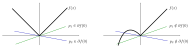
\includegraphics[width=1\textwidth]{./Figures/subdiferencial}
    \caption{Exemplo de subdiferencial. Perceba que considerando
    o subdiferencial generalizado, teríamos
    $p_1 \in \partial_G f(0)$ e $p_2 \in \partial_G f(0)$ para as duas imagens.}
    \label{fig:subdiferencial}
\end{figure}

Agora podemos definir de forma rigorosa o fluxo de gradiente.

\begin{definition}[Fluxo de Gradiente]
    Seja $f:\mathbb R^n \to \mathbb R$.
    Assim, dizemos que $x:(0,+\infty) \to \text{Dom}(f)$ é um fluxo de gradiente
    de $f$ se $x \in \text{AC}_{\text{loc}}((0,+\infty), \mathbb R^n)$ e
    \begin{equation}
        x'(t) \in - \nabla_G f(x(t)), \quad \text{para } \lambda\text{-a.e } t \in (0,+\infty),
    \end{equation}
    onde $\lambda$ é a medida de Lebesgue. Note que dizemos que $x$ começa em $x_0$ se
    $\lim_{t \to 0^+} x(t) = x_0$.
\end{definition}

\subsection{Resultados Básicos de Existência e Unicidade}

Uma vez introduzida a ideia de fluxo de gradiente, vamos agora provar alguns
resultados básicos relacionados ao sistema de equações

\begin{equation}
    \begin{cases}
        x'(t) \in -\partial F(x(t)), \ \text{para quase todo } t>0,\\
        x(0)  = x_0.
    \end{cases}
    \label{eq:fluxograd}
\end{equation}

Veja que agora a função $F$ não é mais necessariamente derivável. Este cenário
é bem menos restrito que o que apresentamos logo no início do capítulo.

\begin{lemma}
    Seja $f:\mathbb R^n \to \mathbb R \cup \{+\infty\}$ convexa, $p_1 \in \partial f(x_1)$
    e $p_2 \partial f(x_2)$. Então
    \begin{equation}
        \langle p_1 - p_2, x_1 - x_2 \rangle \geq 0.
    \end{equation}
\end{lemma}
\begin{prf}
    Pela definição de subdiferencial, temos que
    \begin{align*}
        &p_1 \in \partial f(x_1) \implies f(x_2) \geq f(x_1) + \langle p_1, x_2 - x_1\rangle\\
        &p_2 \in \partial f(x_2) \implies
        f(x_1) \geq f(x_2) + \langle p_2, x_1 - x_2\rangle.
    \end{align*}
    Assim, somando as duas equações, temos que
    \begin{align*}
        &f(x_2) + f(x_1) \geq f(x_1) + f(x_2) +
        \langle p_1, x_2 - x_1\rangle
        \langle p_2, x_1 - x_2\rangle
    \end{align*}
    Rearranjando, obtemos
    \begin{align*}
        &0 \geq
        \langle p_1,x_2 \rangle
        -\langle p_2,x_1 \rangle
        \langle p_2,x_1 \rangle
        -\langle p_2,x_2 \rangle \\
        &\implies
        \langle p_1 - p_2 , x_1 - x_2 \rangle \geq 0.
    \end{align*}
\end{prf}

\begin{theorem}
    Seja $F:\mathbb R^n \to \mathbb R$ \textbf{convexa}, $x_0 \in \mathbb R^n$, e
    $x_1$ e $x_2$ duas soluções de \eqref{eq:fluxograd}.
    Então,
    \begin{equation}
        |x_1(t) - x_2(t)| \leq |x_1(0) - x_2(0)|, \ \forall t >0.
    \end{equation}
    Logo, a solução do sistema de equações é única.
\end{theorem}
\begin{prf}
    Primeiro, faça $g(t) = \frac{(x_1(t) - x_2(t))^2}{2}$, e toma a derivada em $t$. Assim
    \begin{equation*}
        g'(t) = \langle x_1(t) - x_2(t), x_1'(t) - x_2'(t) \rangle.
    \end{equation*}
    Usando o fato que
    $x_1'(t) \in \partial F(x_1(t))$ e
    $x_2'(t) \in \partial F(x_2(t))$, temos pelo lemma que acabamos de demonstrar que
    \begin{equation*}
        g'(t) = \langle x_1'(t) - x_2'(t) , x_1(t) - x_2(t) \rangle \geq 0.
    \end{equation*}
    Além disso, como ambas as soluções começam em $x_0$, temos que $g(0) = 0 \geq g(t)$, já que
    a derivada de $g(t)$ é sempre menor ou igual a zero. Portanto
    \begin{align*}
        g(t) = \frac{(x_1(t) - x_2(t))^2}{2} \leq 0 &\implies
        |x_1(t) - x_2(t)| \leq |x_1(0) - x_2(0)| = 0 
        \\
        &\implies
        x_1(t) = x_2(t).
    \end{align*}
\end{prf}

Podemos estender o resultado do teorema acima para o caso mais geral onde
$F$ é $\lambda$-convexa. A demonstração é bastante parecida, porém, um pouco mais convoluta.
Por conta disso optamos por apresentar os dois resultados de forma separada.

\begin{theorem}
    Seja  $F:\mathbb R^n \to \mathbb R$ \textbf{$\lambda$-convexa}, $x_0 \in \mathbb R^n$.
    Então o sistema de equações \eqref{eq:fluxograd} tem uma solução única.
    Além disso, se $\lambda >0$, a taxa de convergência para o mínimo global
    de $F$ é exponencial, ou seja, para $x^* = \argmin_{x\in \mathbb R^n} F(x)$
    \begin{equation}
        |x(t) - x^*| \leq e^{-\lambda t}|x(0)- x^*|,
    \end{equation}
    onde $x(t)$ é a solução.
\end{theorem}

Outra propriedade relevante dos fluxos de gradiente é que eles podem ser
caracterizados por meio do chamado \textit{Esquema de Minimização de Movimento}.
A ideia é a seguinte, imagine que queremos resolver o problema de fluxo de gradiente
descrito em \eqref{eq:fluxograd}. Uma forma de fazer isso seria discretizando
a variável $t$, e aplicando algum método de descida em relação à $F$,
já que $x(t)$ tem ``velocidade'' sempre na direção oposta do gradiente de $F$.
Assim, denotaremos um \textit{time-step} $\tau >0$, e uma sequência $(x_k^\tau)$,
onde $x_0^\tau = x(0)$, $x_1^\tau = x(\tau)$,..., $x_k^\tau = x(k\tau)$, ou seja,
cada elementos da sequência representa um ponto da solução $x(t)$ no tempo discretizado.

O \textit{Esquema de Minimização de Movimento} é definido pela seguinte iteração:
\begin{equation}
    x_{k+1}^\tau \in \argmin_{x} F(x)+\frac{|x - x_k^\tau|^2}{2\tau}.
    \label{EMM}
\end{equation}
Note que se $F$ for $\lambda$-convexa, o problema acima tem solução única.
A primeira vista, o esquema de minimização acima pode parecer contra-intuitivo, entretanto,
supondo que $F$ é derivável, sabemos que a solução de \eqref{EMM} é obtida quando
$\nabla (F(x)+\frac{|x - x_k^\tau|^2}{2\tau})= 0$, assim,
\begin{equation}
    - \nabla F(x_{k+1}^\tau) = \frac{x_{k+1}^\tau - x_k^\tau}{\tau}.
\end{equation}
Ou seja, esse esquema de minimização é o famoso esquema implícito de Euler.
Lembre-se da diferença entre o esquema implícito e o explícito de Euler:
\begin{flalign}
    \text{(Euler Implícito)} && x_{k+1}^\tau = x_k^\tau - \tau \nabla F(x_{k+1}^\tau) &&
\end{flalign}
\begin{flalign}
    \text{(Euler Explicito)} && x_{k+1}^\tau = x_k^\tau - \tau \nabla F(x_{k}^\tau) &&
\end{flalign}

Suponha que queremos achar a solução para o intervalo de tempo $[0,T]$. Assim,
discretizamos esse intervalo em usando o passo $\tau$.
Uma vez que obtemos a sequência de pontos $(x_k^\tau)$, o objetivo agora é interpolar
esses pontos de alguma forma a gerar uma solução aproximada de $x(t)$ para $t \in [0,T]$.
A maneira mais óbvia seria por meio de uma interpolação linear, que denotaremos por
$\tilde x^\tau(t)$. Outra seria fazendo $x^\tau(t) = x_{k+1}^\tau$, ou seja, uma função
escada. Ambos métodos são ilustrados na Figura \ref{fig:eulerinterpolacao}.
\begin{figure}[H]
\begin{center}
    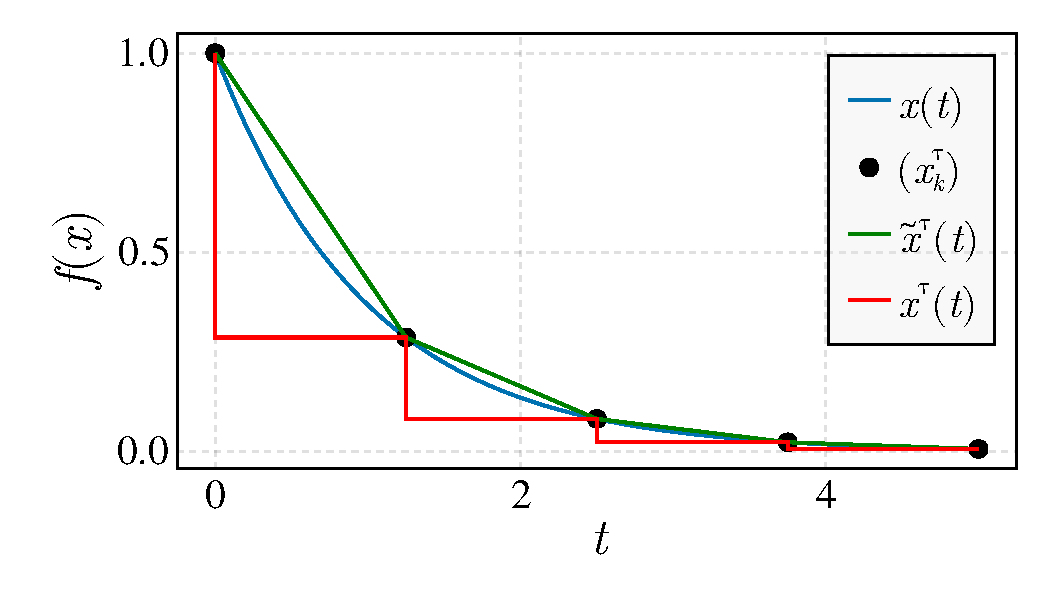
\includegraphics[width=0.6\textwidth]{./Figures/eulerinterpolacao}
\end{center}
    \caption{Exemplo de aproximação da solução $x(t)$ por
    meio de $x^\tau(t)$ usando interpolação linear dos pontos da sequência $(x_k^\tau)$.}
    \label{fig:eulerinterpolacao}
\end{figure}

Agora apresentamos o seguinte resultado que caracteriza o
\textit{Esquema de Movimento de Minimização} \eqref{EMM}
com a solução do fluxo de gradiente.

\begin{theorem}
    Sejam $\tilde x^\tau, x^\tau$ construídas como apresentado acima. Suponha que
    $F(x_0)<+\infty$ e $F(x)>-\infty$ para todo $x$. Então, existe uma subsequência
    $\tau_i \to 0$, tal que ambas aproximações
    $\tilde x^\tau$ e $x^\tau$ convergem uniformemente para $x(t)$ em $[0,T]$, onde $x(t)$
    é Absolutamente Contínua em $[0,T]$ e é $L^2$. Além disso, defina
    \begin{equation}
        \bm v^\tau(t) = \frac{x_{k+1}^\tau - x_k^\tau}{\tau}, \ \text{para } t \in (k\tau,(k+1)\tau].
    \end{equation}
    Assim, $\bm v^\tau$ converge fracamente em $L^2$ para $\bm v = x'$ e
    \begin{enumerate}
        \item Se $F$ é $\lambda$-convexo, então $\bm v(t) \in -\partial F(x(t))$ em quase todo $t$;
        \item Se $F \in C^1$, então $\bm v(t) = - \nabla F(x(t))$ para quase todo $t$.
    \end{enumerate}
\end{theorem}

\section{Fluxo de Gradiente em Espaços Métricos}

Começamos nossa exposição focando em $\mathbb R^n$, porém, espaços de Wasserstein
são espaços métricos geodésicos onde não está claro, por exemplo, o que seria
$x'(t)$ onde $x(t) = \mu_t \in \mathcal P(\mathbb R^n)$.
Assim, vamos estender nossa análise subsequente para o caso de espaços métricos geodésicos.

\subsection{Revisando Geodésicas}

O conceito de geodésicas já foi apresentado no Capítulo anterior. Porém, vamos
fazer uma breve revisão\footnote{Retirar essa seção na versão final do livro. Está aqui
somente para que o capítulo seja mais auto-contido.}.

\begin{definition}[Derivada Métrica]
    Seja $\omega:[0,1] \to X$ uma curva no espaço métrico $(X,d)$. Definimos
    a sua derivada métrica como
    \begin{equation}
        |\omega'|(t) := \lim_{h\to 0}\frac{d(\omega(t+h),\omega(t))}{|h|},
    \end{equation}
    caso esse limite exista.
\end{definition}

\begin{definition}[Curva Absolutamente Contínua]
    Uma curva $\omega:[0,1] \to \mathbb X$ é dita absolutamente contínua se existir
    $g \in L^1([0,1])$ tal que $d(\omega(t_0),\omega(t_1)) \leq \int^{t_1}_{t_0} g(s)ds$ para
    todo $t_0 < t_1$. O conjunto de todas as curvas absolutamente contínuas em $(X,d)$
    é denotado por $\text{AC}(X)$, onde omitimos o $d$ quando a métrica está clara.
\end{definition}

\begin{definition}[Comprimento]
    Seja $\omega:[0,1] \to X$ um curva, defina o comprimento dessa curva como
    \begin{equation}
        \text{Len}(\omega):= \sup\left\{
            \sum^{n-1}_{k=0}d(\omega(t_k),\omega(t_{k+1})): \ n\geq 1,
            0 = t_0 < t_1,...,t_n=1
        \right\}.
    \end{equation}
\end{definition}

\begin{definition}[Geodésica]
    Uma curva $\omega:[0,1]\to X$ é uma geodésica entre $x_0$ e $x_1 \in X$ se
    $\omega(0)=x_0$, $\omega(1)=x_1$ e
    $\text{Len}(\omega) = \min\{\text{Len}(\tilde \omega): \omega \in \text{AC}(X)
    , \tilde \omega(1)=x_1\}$.
    Ou seja, um curva $\omega$ é uma geodésica entre dois pontos caso ela seja a curva
    de menor distância.
\end{definition}
Assim, fica claro que a idéia de geodésica é uma extensão da idéia de retas em espaços
Euclidianos para espaços mais gerais, como superfícies curvas. 

\begin{definition}[Espaço Geodésico]
    Um espaço métrico $(X,d)$ é um espaço geodésico se para todo $x,y \in X$,
    \begin{equation}
        d(x,y) = \min\{\text{Len}(\omega): \omega \in \text{AC}(X), \omega(0)=x, \omega(1)=y\}.
    \end{equation}
    Ou seja, a distância entre dois pontos é dada pela geodésica de menor comprimento.
    Note que num espaço geodésico, essa geodésica sempre existe.
\end{definition}

\begin{definition}[Geodésica de Velocidade Constante]
    Uma geodésica $\omega:[0,1]\to X$ é dita ter velocidade constante se
    \begin{equation}
        d(\omega(t), \omega(s)) = \frac{|t-s|}{1 - 0} d(\omega(0),\omega(1)), \forall t,s \in [0,1].
    \end{equation}
\end{definition}

O Teorema [\ref{theorem.AC_metric_derivative}] mostra que para curvas $\omega \in \text{AC}(X)$, temos
que
\begin{equation}
    \text{Len}(\omega) = \int_0^1 |\omega '|(t) dt,
\end{equation}
ou seja, se $\omega$ for de velocidade constante, temos que $\omega'(t)$ é
a velocidade de $\omega$ e é uma constante.

Vamos mostrar agora que na verdade toda geodésica pode ser reparametrizada
para possuir velocidade constante.

\begin{proposition}
    Seja $(X,d)$ um espaço geodésico. Então, para todo $x_1,x_2 \in X$,
    existe uma geodésica de velocidade constante $\tilde \omega(t)$ ligando
    $x_1$ e $x_2$, i.e. $\tilde \omega(0) = x_1$ e $\tilde \omega(1) = x_2$.
\end{proposition}
\begin{prf}
    Seja $\omega(t)$ uma geodésica entre $x_1$ e $x_2 \in X$, teremos então
    \begin{equation*}
        d(x_1,x_2) = \text{Len}(\omega) = \int_0^1 |\omega'|(t)dt.
    \end{equation*}
    Faça agora $\tilde \omega (s) = \omega(g(s))$, onde
    \begin{equation*}
        g(s):= \bar r_s \cdot d(x_1,x_2),
    \end{equation*}
    onde
    \begin{equation*}
        \bar r_s := \inf \left\{
            r \in [0,1]: \int^r_0 |\omega'|(t) dt\geq s
            \right\}
    \end{equation*}
    Assim, $\text{Len}(\tilde \omega) = d(x_1,x_2)$ e tem velocidade constante.

    \textbf{Exercício. Conclua demonstrando que de fato essa curva $\tilde \omega$ tem comprimento
    igual à $\omega$ e tem velocidade constante. Pensei nessa solução, mas não cheguei a verificar
    se de fato é verdade.}
\end{prf}

Concluímos essa revisão de geodésicas com uma definição menos comum, chamada de convexidade geodésica.

\begin{definition}[Convexidade Geodésica]
    Seja $(X,d)$ um espaço geodésico. Assim, a função $F:X \to \mathbb R \cup \{+\infty\}$
    é \textit{geodesicamente convexa} se para todo $x_0,x_1 \in X$, existe uma geodésica
    de velocidade constante $x(t)$
    entre $x_0$ e $x_1$, onde a função $F$ é convexa, ou seja,
    \begin{equation}
        F(x(t)) \leq (1-t)F(x(0)) + tF(x(1)).
    \end{equation}
    E, similarmente, $F$ é dita \textit{geodesicamente $\lambda$-convexa} se
    \begin{equation}
        F(x(t)) \leq (1-t)F(x(0)) + tF(x(1))-\lambda\frac{t(1-t)}{2}d^2(x_0,x_1).
    \end{equation}
    Note que essa definição na verdade é mais fraca que convexidade ao longo de toda geodésica,
    pois, é possível que existam duas geodésicas entre $x_0$ e $x_1$, onde $F$ é convexa
    em uma, mas não é na outra.
\end{definition}



% \begin{theorem}
% 	\label{thm:acmetricderivative}
% 	Seja $(X,d)$ um espaço métrico separável e limitado. Então,
%     para todas as curvas AC $\omega :[0,1] \to X$
% 	\begin{equation*}
% 	|\dot{\omega}|(t) := \lim_{h \to 0} \frac{d(\omega(t+h), \omega(t))}{h}.
% 	\end{equation*}
% 	existe $L^1([0,1])$-q.p., a função $t \mapsto |\dot{\omega}|(t)$ é integrável e
%     $|\dot{\omega}|(\cdot)$ é o módulo de integração mínimo de $\omega$, o que implica que
% 	\begin{equation}
% 	d(\omega(t),\omega(s)) = \int_s^t |\dot{\omega}|(r)\dd r.
% 	\end{equation} 
% \end{theorem}

\subsection{Formulação EDE e EVI}

Considere um espaço métrico $(X,d)$, com $F:X\to \mathbb R\cup{+\infty}$ inferiormente
semi-continua. Assim, o \textit{Esquema de Minimização de Movimento} pode ser
reescrito como
\begin{equation}
    x_{k+1}^\tau \in \argmin_x F(x) + \frac{d(x,x_k^\tau)^2}{2\tau}.
    \label{metricEMM}
\end{equation}

Sendo nosso espaço geodésico, podemos usar novamente a idéia de obter
uma sequência de pontos $(x_k^\tau)$, e obter $x^\tau(t)$ interpolando com geodésicas.
Ou seja, para $t \in (k\tau,(k+1)\tau]$, faça $x^\tau(t)$ igual a geodésica
de velocidade constante $d(x_k^\tau,x_{k+1}^\tau)/\tau$, que sempre existirá se
nosso espaço for geodésico.

Queremos assim que $x^\tau$ convirja para uma solução $x(t)$ onde
$x'(t) = -\nabla F(x(t))$. Porém, para um espaço métrico qualquer
não está claro que nem $x'(t)$ nem $-\nabla F(x(t))$ existem!
Invés disso podemos usar a noção de derivada métrica que apresentamos e
que sabemos que de fato existirá.

